%! alt Isosceles triangle ACE with CA = CE = h, drawn for h = 144. B is the midpoint of AE, with AB = BE = 90 and a right angle between BC and AE. D lies on side CE, and AD bisects angle CAE. CB bisects angle ACE, so E is the reflection of A in line BC.
%! after_paragraph 3
%! scale 1/23
% The shared preamble of every Kyuclid figure. pipeline/figures turns these colours into theme-aware paint,
% and refuses any other colour, so draw only with them:
%   figink (lines and labels), figaux (construction lines), figaccent (the object the argument turns on),
%   figtint and figaccenttint (light fills).
\documentclass[border=1.5pt]{standalone}
\usepackage{tkz-euclide}
\definecolor{figink}{RGB}{0,0,0}
\definecolor{figaux}{RGB}{85,85,85}
\definecolor{figaccent}{RGB}{192,57,43}
\definecolor{figtint}{RGB}{221,221,221}
\definecolor{figaccenttint}{RGB}{245,213,208}
% tkz-euclide's defaults draw circles, compasses and marks in 50% grey and fill points with a tint.
\makeatletter
\def\tkz@otherlinecolor{figink}
\def\tkz@euc@circlecolor{figink}
\def\tkz@euc@compasscolor{figink}
\def\tkz@euc@mkcolor{figink}
\def\tkz@mk@fill{figink}
\def\tkz@euc@pointfillcolor{figink}
\makeatother
\tkzSetUpLine[color=figink,line width=.7pt]
\tkzSetUpArc[color=figink,line width=.7pt]
\tkzSetUpCompass[color=figink,line width=.5pt]
\tkzSetUpPoint[color=figink,fill=figink,size=3.1pt]
\tikzset{
  every picture/.style={line cap=round,line join=round,color=figink},
  circle style/.append style={color=figink,line width=.7pt},
  aux/.style={color=figaux,line width=.45pt,dash pattern=on 2.6pt off 2pt},
  key/.style={color=figaccent,line width=1pt},
  mk/.style={color=figink,line width=.5pt},
  lbl/.style={color=figink,inner sep=2.2pt},
  len/.style={color=figink,inner sep=1.5pt,font=\small},
}

\begin{document}
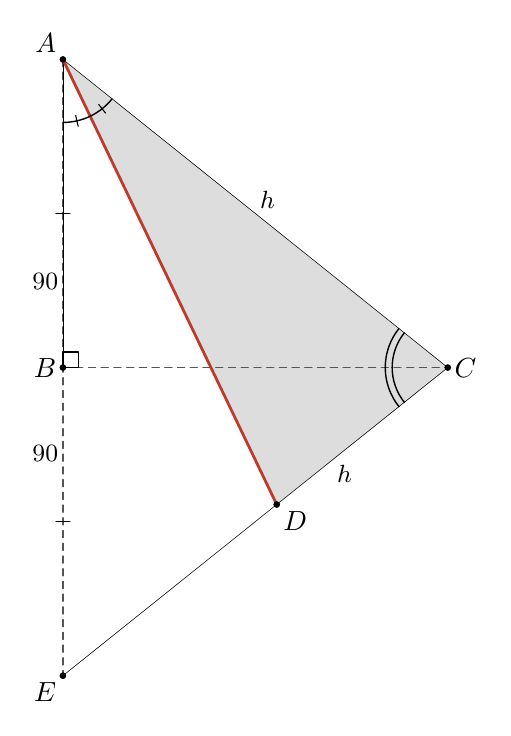
\begin{tikzpicture}
\tkzDefPoint(0.0,0.0){B} %! B = (0, 0)
\tkzDefPoint(0.0,3.9130435){A} %! A = (0, 90)
\tkzDefPoint(0.0,-3.9130435){E} %! E = reflect(A, B, (1, 0))
\tkzDefPoint(4.8873897,0.0){C} %! C = (sqrt(144**2 - 90**2), 0)
\tkzDefPoint(2.7152165,-1.7391304){D} %! D = lerp(C, E, 144/(144 + 180))
%! fact dist(A, B) == 90
%! fact dist(A, E) == 180
%! fact perp(A, E, B, C)
%! fact dist(C, A) == 144
%! fact dist(C, E) == 144
%! fact on_segment(D, C, E)
%! fact angle(B, A, D) == angle(D, A, C)
%! fact angle(A, C, B) == angle(B, C, D)
%! fact dist(C, D) == 144**2/(144 + 180)
\tkzFillPolygon[color=figtint](A,C,D)
\tkzDrawSegment[aux](A,E)
\tkzDrawSegment[aux](B,C)
\tkzDrawSegments(A,C C,E)
\tkzDrawSegment(A,B)
\tkzDrawSegment[key](A,D)
\tkzMarkRightAngle[size=.2,mk](C,B,A)
\tkzMarkSegments[mark=|,size=2.5pt,mk](A,B B,E)
\tkzMarkAngles[size=.8,arc=l,mark=|,mksize=2pt,mk](B,A,D D,A,C)
\tkzMarkAngles[size=.75,arc=ll,mark=none,mk](A,C,B)
\tkzMarkAngles[size=.75,arc=ll,mark=none,mk](B,C,D)
\tkzDrawPoints(A,B,C,D,E)
\tkzLabelPoint[above left,lbl](A){$A$}
\tkzLabelPoint[left,lbl](B){$B$}
\tkzLabelPoint[right,lbl](C){$C$}
\tkzLabelPoint[below right,lbl](D){$D$}
\tkzLabelPoint[below left,lbl](E){$E$}
\tkzLabelSegment[above right,len](A,C){$h$}
\tkzLabelSegment[below right,pos=.3,len](C,E){$h$}
\tkzLabelSegment[left,pos=.72,len](A,B){$90$}
\tkzLabelSegment[left,pos=.28,len](B,E){$90$}
\end{tikzpicture}
\end{document}
